
%###################################### Packages and new functions definitions ###########################################%
%Encoding Package
\documentclass[11pt]{sample}
\usepackage{pslatex}
%\usepackage[latin1]{inputenc}
%\usepackage[francais]{babel}
\usepackage[T1]{fontenc}
\usepackage{fancybox}
\usepackage{a4wide}
\usepackage[toc]{appendix}
\usepackage{CJK}
\newcommand\japonais[1]{\begin{CJK*}{UTF8}{song}#1\end{CJK*}}
\usepackage{color}
%Type de package de couleur : au choix. Attention n'en choisir qu'un seul à  la fois
%\usepackage{xcolor}
%\usepackage[dvipsnames]{xcolor}
\usepackage[svgnames]{xcolor}

%Packages Algoritmic
\usepackage{algorithm}
\usepackage{algorithmic}

%Packages Images & graph
\usepackage{graphicx}
\usepackage{graphics}
\graphicspath{{./images/}}
\bibliographystyle{prsty}

\renewcommand{\algorithmicrequire} {\textbf{\textsc{\textcolor{DarkSlateGray}{In:}}}}
\renewcommand{\algorithmicensure}  {\textbf{\textsc{\textcolor{DarkSlateGray}{Out:}}}}
\renewcommand{\algorithmicwhile}   {\textcolor{DarkOrchid}{\textbf{While}}}
\renewcommand{\algorithmicdo}      {\textcolor{DarkOrchid}{\textbf{Do}}}
\renewcommand{\algorithmicendwhile}{\textcolor{DarkOrchid}{\textbf{End While}}}
\renewcommand{\algorithmicend}     {\textcolor{DarkOrchid}{\textbf{End}}}
\renewcommand{\algorithmicif}      {\textbf{\textcolor{DarkOrchid}{If}}}
\renewcommand{\algorithmicendif}   {\textcolor{DarkOrchid}{\textbf{End If}}}
\renewcommand{\algorithmicelse}    {\textcolor{DarkOrchid}{\textbf{Else}}}
\renewcommand{\algorithmicthen}    {\textcolor{DarkOrchid}{\textbf{Then}}}
\renewcommand{\algorithmicfor}     {\textbf{\textcolor{DarkOrchid}{For}}}
\renewcommand{\algorithmicforall}  {\textbf{\textcolor{DarkOrchid}{For All}}}
\renewcommand{\algorithmicdo}      {\textbf{\textcolor{DarkOrchid}{Do}}}
\renewcommand{\algorithmicendfor}  {\textbf{\textcolor{DarkOrchid}{End For}}}
\renewcommand{\algorithmicloop}    {\textbf{\textcolor{DarkOrchid}{Loop}}}
\renewcommand{\algorithmicendloop} {\textbf{\textcolor{DarkOrchid}{End Loop}}}
\renewcommand{\algorithmicrepeat}  {\textbf{\textcolor{DarkOrchid}{Repeat}}}
\renewcommand{\algorithmicuntil}   {\textbf{\textcolor{DarkOrchid}{Until}}}
\renewcommand{\algorithmicreturn}  {\textbf{\textcolor{DarkOrchid}{return}}}
\newcommand{\algorithmicelseif}{\textbf{\textcolor{DarkOrchid}{Elsif }}}
%\floatname{algorithm}{Algorithme}
\let\mylistof\listof
\renewcommand\listof[2]{\mylistof{algorithm}{List of algorithm}}



\makeatletter
\providecommand*{\toclevel@algorithm}{0}
\makeatother
\makeatletter
\def\clap#1{\hbox to 0pt{\hss #1\hss}}%
\def\ligne#1{%
  \hbox to \hsize{%
    \vbox{\centering #1}}}%
\def\haut#1#2#3#4{%
  \hbox to \hsize{%
    \rlap{\vtop{\centering #1}}%
    \rlap{\vtop{\centering #2}}%
    \clap{\vtop{\centering #3}}%
    \llap{\vtop{\centering #4}}}}%
\def\bas#1#2#3{%
  \hbox to \hsize{%
    \rlap{\vbox{\raggedright #1}}%
    \hss
    \clap{\vbox{\centering #2}}%
    \hss
    \llap{\vbox{\raggedleft #3}}}}%
\def\maketitle{%
  \thispagestyle{empty}\vbox to \vsize{%
    \haut{}{\@blurb}{}
    \vfill
    \vspace{4cm}
    \ligne{\Large \@title}
    \vspace{5mm}
    \ligne{\Large \@author}
    \vspace{1cm}
    \vfill
    \vfill
    \bas{}{\hspace{20mm} \@location, \@date\newline}{}
  }%
  \cleardoublepage
}
\def\date#1{\def\@date{#1}}
\def\author#1{\def\@author{#1}}
\def\title#1{\def\@title{#1}}
\def\location#1{\def\@location{#1}}
\def\blurb#1{\def\@blurb{#1}}
\def\email#1{\def\@email{#1}}
\def\logo#1{\def\includegraphics[height=3\baselineskip]{#1}}
\date{\today}
\author{}
\title{}
\location{Ichinoseki Kousen}
\blurb{}
\email{steeve.vandecappelle@free.fr}
\makeatother
\title{\begin{Huge}\textcolor{blue}{Project: Ichiman Yen}\end{Huge}}
\author{Vandecappelle  \textsc{Steeve} }
\date{From 30th march to 28th Juin 2009}
\location{Ichinoseki}
\blurb{  \hspace{1mm}
\includegraphics[height=3\baselineskip]{iutaustl.jpg}\hspace{100mm}
\includegraphics[height=3\baselineskip]{ichinoseki-koosen.jpg}\\
  Insititut Universitaire de Lille 1 \\
  Ichinoseki kousen \\[1em]
  Placement Report\\\vspace{4mm}
  tutors:\\
  Obokata-sensei and Kaname-sensei\\
}







%#################################################### Beginning document #################################################%
\begin{document}
\maketitle
\newpage
\strut
\newpage
\startcontents[sections]
%####################################################### Contents ########################################################%
\section*{Contents} 
\printcontents[sections]{l}{1}{\setcounter{tocdepth}{2}}
\newpage

%#################################################### Thanks Section #####################################################%
\section*{Thanks \markboth{Thanks}{Thanks}}
\addcontentsline{toc}{section}{\protect\numberline{}Thanks} 
First I wish I would to thank Mr. Koichi the principal of the Ichinoseki national college and the administrative team for giving me a good reception.
\\Second I wish I would to thank people who help me during the placement, Mr Obokata, Mr Kaname, Mr Chiba,  and also the 5S classroom's students especially Henhee, Miyuki and Takehana.
\\Finally I wish I would to thank the people who helped me for the language, Mr Rigal, Mr Lebegue, Miss Aki,Tchai, Pakusan, Azelin, and Moyo.
\\\vspace{2mm}
This placement is the result of my two years of studied in the Technological University Insitute of Lille 1 in computer-science. I hope you will enjoy to learn all of steps of the project.And thank the reader for every comments he would say.Contact me for all questions or comments about the report, the project or the placement.\\
\vspace{15mm}
\japonais{}\\
\section*{\japonais{礼状}}
\japonais{まず 私は 一関高専の 校長先生に お礼 を 言いたい。 そして 私の チューター 小保方先生 と 佐藤 要先生  お礼 を 言いたい です。
\\みなさんが 私を 助けてくれました。
\\それに 私は 5Sの 学生に 楽しい 思いで を ありがとう と 言いたい。ことに 幸と 宮俊介と 竹花 幸伸。 \\
}
\newpage
%################################################### Abstract Section ####################################################%
\section*{Abstract \markboth{Abstract}{Abstract}}
\addcontentsline{toc}{section}{\protect\numberline{}Abstract} 
This project, wich I have done at Ichinoseki, had the aim of give a software, the most easier and the most empty it could it be on the "Ichiman yens" game. So, that's why I do my priority of the Interface graphical-mode, for more lisibility and facility for the users.This project had two axes mandatory: first it would be a C program-coded, and second it had to be a client/server application.\\
\\In the first hand my work consisted of to make a graphical-mode of the server program. The server display the result of each round of the game. For this part of the project, I'd just used the C standard Library and Gtk2.0 Library to obtains the graficals objects necessary. 
\\ On the other hand I wanted to create an other program of reference to do every things the game needs.For create C program, compile them, and execute them. Because of the length of the project I used the Glade Library to gain time and only programing the important code, and don't code all the graphicals declarations, which it would took a long time.
This program contains also a help section, for beginners and non-programer.\\At the end, the window application was able to create C program easily, compile and execute them on the server top level window.

\section*{\japonais{抄録}}
\japonais{この けんしゅうは 私の二年のだいがくの まとめです。\\
私の けんきゅうに 一関の先生は 期待していました。
\\
この けんしゅうの さいしゅう もくてきは グラフィック アプリケーションの 一万円 ゲームを 作ることで、
私は この  アプリケーションの プログラムを 考えました。


}


\newpage
%############################# Présentation du jeu #########################%
\section{General game-introduction}
\subsection{Rudiments of Ichiman game}
Ichiman-game is a strategic game, wich it oppose two players. At the beginning the players have the same numbers of points, 10.000. The game is simple, each players place a bet but they don't know the ennemy's bet. The player had minus bet win the two bet on the table. The round finish when the 10 matchs are played, and all 10.000 yens must have been played. The following picture represent one round of the game: 
\begin{center}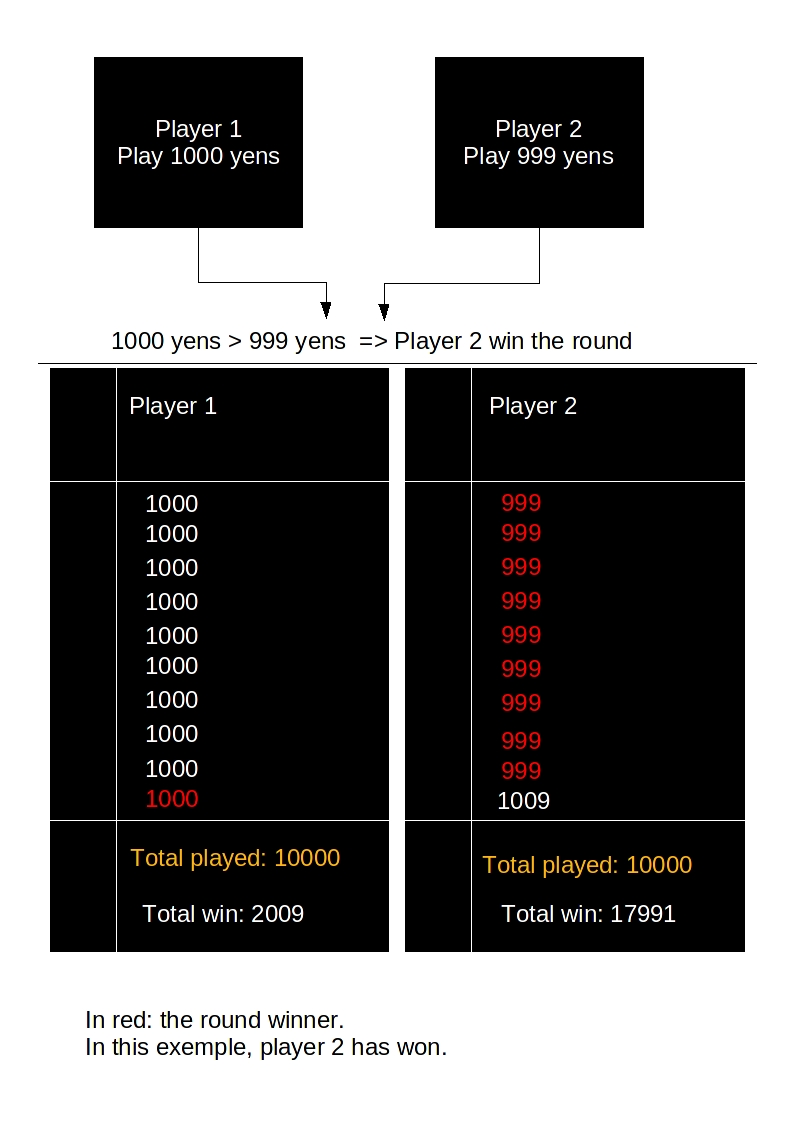
\includegraphics[height=35\baselineskip]{img/match_round_model.jpg}\end{center}
\subsection{Client's programs}
The client's programs is the player representation, it must bet. For each match of a round, it must be return a value to bet on the standard output: "stdout". And the server waits the clients' bet before launch the next match. This is the Server program wich run the two clients'program in others processes. The following algorithm is an exemple of client's program, It just bet 1000 for each match of rounds.

\begin{algorithm}
  \caption{Client's programs:Allways 1000 yens}
  \begin{algorithmic}
    \REQUIRE Integer : numbers\_of\_rounds
    \ENSURE EXIT\_SUCCESS
    \vspace{2mm}
    \STATE \textcolor{ForestGreen}{integer}: \textcolor{Goldenrod}{i}, \textcolor{Goldenrod}{j};\\
    \algorithmicfor{ i  \textbf{\textcolor{DarkOrchid}{ From }} 1  \textbf{\textcolor{DarkOrchid}{To}} numbers\_of\_rounds} 
    \algorithmicdo \\
    \hspace{4mm}\algorithmicfor{ j \textbf{\textcolor{DarkOrchid}{ From }} 1  \textbf{\textcolor{DarkOrchid}{To}} 10} 
    \algorithmicdo \\
    \hspace{8mm}
    \textcolor{Maroon}{/*Display on Standard output (1000)*/}\\    \hspace{8mm}
    Print(1000);\\    \hspace{8mm}
    \textcolor{Maroon}{/*Drain the display-buffer */}\\    \hspace{8mm}
    Flush();\\    \hspace{8mm}
    \textcolor{Maroon}{/*Server's response... Wait for the next round*/}\\    \hspace{8mm}
    Scanf();\\
    \hspace{4mm}\algorithmicendfor\\
    \algorithmicendfor\\
    \STATE \textbf{\textcolor{DarkOrchid}{Return}} EXIT\_SUCCESS;
  \end{algorithmic}
\end{algorithm}
\newpage
\subsection{Server Program}
The Server program must run the two opposing client's programs and display the result of the clash.\\ Then it must redirect the standards input-output for processes communications. The Server is the main program, it needs some arguments for generate the game. These arguments are given by the commands's line argument-chain. \\The Server program must create two new processes, and then run the two clients programs. See the appendix  for know the general algorithm of this program. After creating processes, it scan the standard input (wich it be redirected by pipes\footnotemark). then It send a return value to the clients programs for finished the turn process.
\footnotetext{pipe: A pipe is a communication system. You can send informations at boths ends of a pipe. Indeed, the first is for send and the second is for listen. Two processes can send informations by these pipes. The first processus write into the pipe, while the second listen.}
\\The following pattern swow how the server's communication diagram.
\begin{center}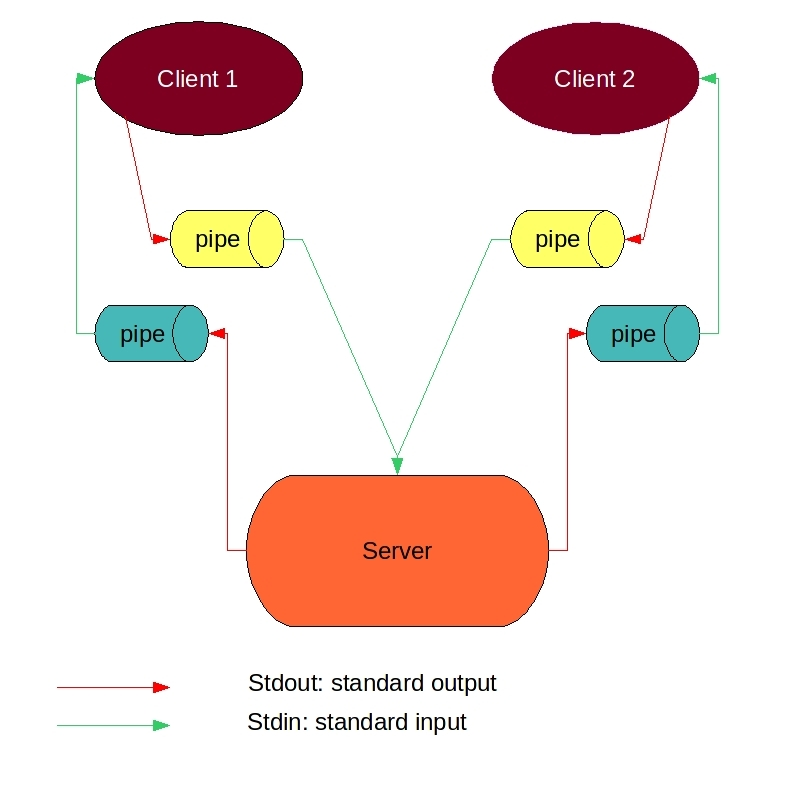
\includegraphics[height=22\baselineskip]{img/pipe_model.jpg}
\end{center}
\newpage
%########################## Partie II L'interface graphique ###########################%
\section{Project with the gtk+2.0 graphical library}
The graphic's devloppment in C language needs a graphical-object's library.That's why I used a library using the GNOME technology of UNIX's systems.
\\For the graphical mode, an object language is necessary to create a type-architecture using extends and implements operations. But C language doesn't include the object, that's why Gtk is a special library. All Gtk's types are typed as GtkWidget, and we can write specific object using functions.Gtk use exclusively pointer's arithmetic then in your program there are no type declared, but only pointers to his memory address.The initalization's function create the specified type for you and just return is memory-map's address.For Exemple:\\
\begin{verbatim}
GtkWidget *window;
Gtkwidget *label;
window = gtk_window_new(GTK_WINDOW_TOPLEVEL);
label = gtk_label_new("a label");
\end{verbatim}
An other important part of Gtk is Macros\footnotemark \ if the type must be used a specific name (in specials functions for exemple) The Gtk's macro make a conversion for the object has specific visibility. For exemple the update-label's function of GtkLabel needs a GtkLabel for first parameter :\\

\begin{verbatim}
GtkWidget *label;
label = gtk_label_new("a label");
gtk_label_set_text(GTK_LABEL(label), "a new text label");
\end{verbatim}
With Macro and Widget's functions, you can create all object as you need for your graphical window. You may use the big list of type and the layers' configurations for create a complex grafic's user interface.However Gtk is limited because of the C language, which you can't create new graphics objects. 

\subsection{Server's display program}
This program serve as the basis of the project. It consist of taking the place of the tutor's server-program. And this program would be an possible improvement of the server but the main server program is existing yet. So you can use the "Terminal" mode yet.\\ That's why, as lots of complex program I used a temporary file for don't re-implement the server's code. The following graph is a main-program behavior's representation.
\footnotetext{Macros: A macro is an abbreviation for a set of commands, so instead of typing a complicated sequence of commands you can simply type the macro's name(Writen in huppercase). You can either think of macros as a new commands in their own right or as subroutines.}
\newpage
\begin{center}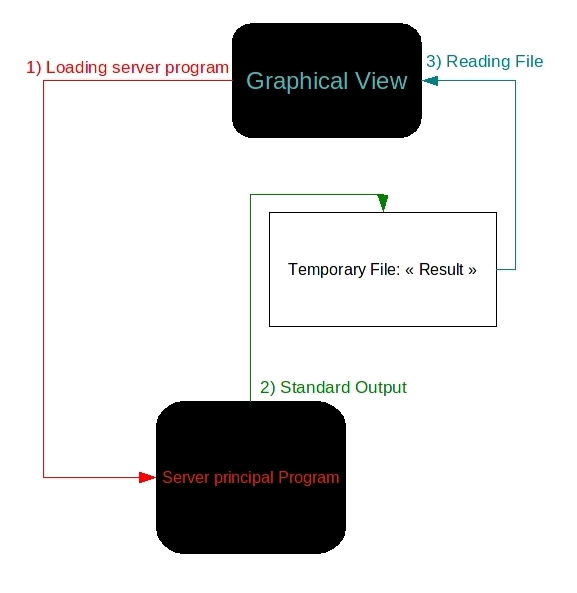
\includegraphics[height=22\baselineskip]{img/GraphicalView-diagram.jpg}\end{center}
The "game" executable break the temporary file down, in some digitals variables for implements the new display. Because of the architecture of these programs, the memory space to allocate can be quite huge if you do more than 500 rounds. So for speed gain the allocation function must taken a high number for don't call this system function for each round. The most important difficulty of this program was to break the program into a few functions, that's why I do 3 main functions. First, to open and read the temporary file into a local variable. Second, find the "n" number of round into this char* variable. And last, find the final winner of the game. You can find these algorithms in appendix. 
\newpage
\subsection{Development's program}
The development's program is the second part of the project and the biggest program.\\ 
Infortunatly, you had to program your clients program with another program. That's why I implemented this section. The aim: "Don't need any other program to play the game." then data are saved in ".c" files and executable can be created.\\
It is the normal entry point of Ichimanyen game and all functions are accessible by execute it. Functions of this program had been created an easy interface of programming. So this program have 3 parts, first you can execute the game display interface. Second, you can create new C program file easily. And last you can compile the your game strategy before execute it.
\subsubsection{Linking of server's display and development's program}
The development's program is like a front office system. You have the heart wich calculate, and the interface wich displays the result you want. The following graphics represent the actions done when you click on "Execute". (The temporary file source does not appear because explained before)
\begin{center}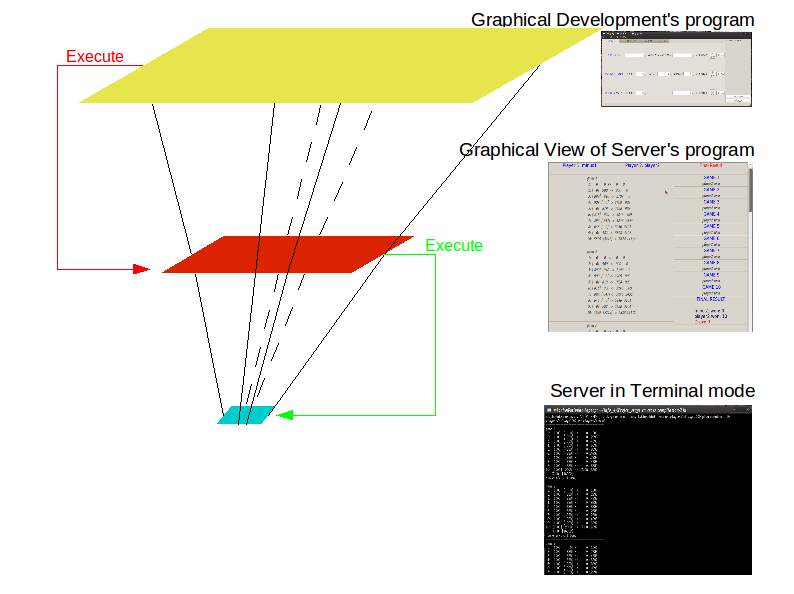
\includegraphics[height=22\baselineskip]{img/Graph_IDE_Representation.png}\end{center}
\subsubsection{Text Editor}
The project was to program in C the clients program, that's why I wanted to keep the C programming aspect. And an integreted-editor was the best thing to keep this aspect.\\
For this part, the text editor is implemented in a new notebook of the main window, for easily switch between compiler, easy coder, and text-editor. Then I will explain the layer system of the text editor: First there is the Notebook where there are all objects about the text editor.\\After a layer is necessary to align all of these objects. First the Editing-Text zone (GtkTextView) and second a toolbar (No buttons on it, but may the aim of an update).In Gtk for insert a new child you must to insert it in a container type. It is an object which can have one or more child. For exemple Notebook is a container (window type) and a GtkBox is also a container (Layer type).But lots of container can't have more than one child, so you must insert into these containers another container which it can received lots of child. Here NoteBook can received only one child, so insert a Layer, and then insert child into this layer.\\ the following picture represent the NoteBook architecture.
\begin{center}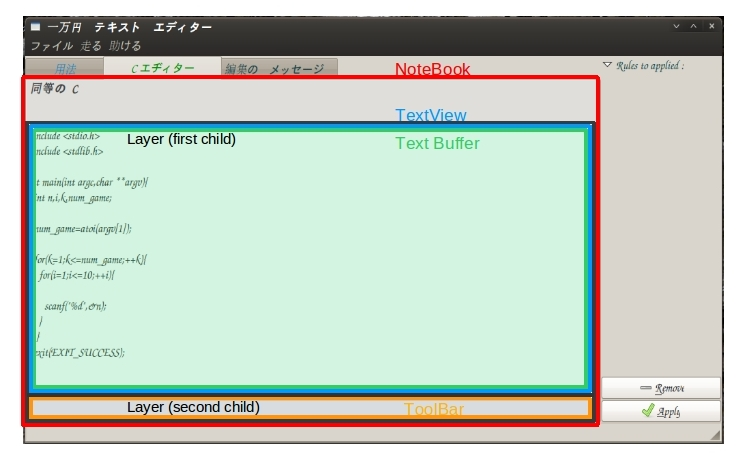
\includegraphics[height=22\baselineskip]{img/Layer-Architecture.jpg}\end{center}
\begin{tiny}*TextBuffer can received a child of the specified type TextBuffer.(It contains the text you have typed.)\end{tiny}
\subsubsection{Files options}
During the project, saving file was important for don't rewrite the code at each new game.\\
 The saving file system is clever program, indeed if you mistaken about the name of the file a warning apear and if you forget to precise the extension of file, the program add it for you. In addition you can save fast your C file juste by typing on keyboard "Ctrl+s". 
\subsubsection{Integreted Compiler}
For easy compile (espacially if running on windows), a compiler is integrated. After saving your project, you can compile it easilly with the Menubar or by typing "Ctrl+Shift+C". This part used the Cross-Compilation Macro for found your default compiler\footnotemark.\footnotetext{See third part of this report for informations about Macros of Cross-compilation}
 The Compile chain is separated in 2 step, first file compile, and second link edition (Executable will be created) these two step are represented in the compiler Text-View, and you may see the errors of compiler because the standard errors output is redirected to the text-view.\\\\
\textcolor{Navy}{Compiler Algorithm\footnotemark}
\begin{algorithm}
  \caption{Compiler Algorithm}
  \begin{algorithmic}
    \REQUIRE TextView\\
    \algorithmicif{ \textcolor{SlateBlue}{File is ever saved}}
    \algorithmicthen{ \\  \hspace{4mm} \textcolor{SlateBlue}{ New Processus}}\\
    \hspace{4mm}\algorithmicif{ \textcolor{Red}{Son Processus} }\algorithmicthen\\
    \hspace{8mm} \textcolor{Red}{Redirect standard error output.}\\
    \hspace{8mm} \textcolor{Red}{Execute Compiler Command.}\\
    \hspace{4mm}\algorithmicelse\\
    \hspace{8mm} \textcolor{SlateBlue}{ Scan on standard input... and verify no errors.}\\
    \hspace{8mm}\algorithmicif{ \textcolor{SlateBlue}{ compiler errors }}\algorithmicthen\\
    \hspace{12mm \textcolor{SlateBlue}{display errors on TextView.}}\\
    \hspace{8mm}\algorithmicelse\\
    \hspace{12mm} \textcolor{SlateBlue}{display no errors on TextView.}\\
    \hspace{12mm} \textcolor{SlateBlue}{ New Processus}\\
    \hspace{12mm}\algorithmicif{ \textcolor{Teal}{Son Processus} }\algorithmicthen\\
    \hspace{16mm} \textcolor{Teal}{ Redirect standard error output.}\\
    \hspace{16mm}  \textcolor{Teal}{Execute Liker Command and create executable.}\\
    \hspace{12mm}\algorithmicelse\\
    \hspace{16mm} \textcolor{SlateBlue}{ Scan on standard input... and verify no errors.}\\
    \hspace{16mm}\algorithmicif{  \textcolor{SlateBlue}{compiler errors} }\algorithmicthen\\
    \hspace{20mm} \textcolor{SlateBlue}{display errors on TextView.}\\
    \hspace{16mm}\algorithmicelse\\
    \hspace{20mm} \textcolor{SlateBlue}{display no errors on TextView.}\\
    \hspace{16mm}\algorithmicendif\\
    \hspace{12mm}\algorithmicendif\\
    \hspace{8mm}\algorithmicendif\\
    \hspace{4mm}\algorithmicendif\\
    \algorithmicendif
    
  \end{algorithmic}
\end{algorithm}
\footnotetext{\\ \textcolor{SlateBlue}{In blue: The first processus, main processus(ichiman-game)}\\ \textcolor{Red}{In red: The first son processus, compiler processus 1(separated file compilation)}\\ \textcolor{Teal}{In green: The Second son processus, compiler processus 2 (link editions)}}
\subsubsection{Easy C code-editor }
This section was created to enable somebody to play ichiman-game even if he/she don't know C language.He just must to select the rules he wants to apply to the project and then in the text-editor the c code will appear. Lots of controls and warnings will appear if some rounds rules seems to be false (For exemple: if some rounds are not implemented or if total bet is less or more than 10.000).\\
The datas processing is sequential, it means that your first selected rule is the first implemented. \\Three function are used for information translating.\\
\textcolor{Navy}{First is the sequential scan of the list:}\\
\begin{algorithm}
  \caption{Sequential scan}
  \begin{algorithmic}
    \REQUIRE \textcolor{ForestGreen}{GtkBox*} \textcolor{Goldenrod}{rules\_box}\\
    \algorithmicif{ list is empty }\algorithmicthen\\
    \hspace{4mm}error message\\
    \algorithmicelse\\
    \hspace{4mm}\algorithmicwhile{ List is not empty }\\
    \hspace{8mm}Apply Rule List (i) \textcolor{Sienna}{ /*(Rules were contained in the GtkBox passing in parameter)*/}\\
    \hspace{4mm}\algorithmicendwhile\\
    \hspace{4mm}\algorithmicif{ total Yens different of 10.000 }\algorithmicthen\\
    \hspace{8mm}display warnings\\
    \hspace{4mm}\algorithmicendif
    \algorithmicendif
  \end{algorithmic}
\end{algorithm}\\
\textcolor{Navy}{Second is the C program TextView updater:}\\
\begin{algorithm}
  \caption{Sequential scan}
  \begin{algorithmic} 
    \REQUIRE\textcolor{DarkOrchid}{const} \textcolor{ForestGreen}{char*} \textcolor{Goldenrod}{Rule\_Label}\\
    \algorithmicif{ rule is "From x To y" Rule }\algorithmicthen\\
    \hspace{4mm}Get and Apply Rule Code function.\\
    \algorithmicelseif{rule is "For x" Rule }\algorithmicthen\\ 
    \hspace{4mm}Get and Apply Rule Code function.\\
    \algorithmicelse\\
    \hspace{4mm}Get and Apply Rule Code function.\\
    \algorithmicendif
  \end{algorithmic}
\end{algorithm}\\
\textcolor{Navy}{And Last is the c code generator:}\\
The code generator-functions just extract the 2 or 3 important informations: Round Begining (Or round modulo number), Round of the end (Can be null for "Modulos" and "For x" rules), and the bet you want. And then it insert these information beetween C language before return the String would be added to the TextView of text-editor notebook. 
\newpage
%########################## Partie III la cross Compilation et les aides intégré dans l'interface graphique ##############%
\section{Cross-compilation and help files}
When the graphical view was finished I found the idea of going on further this universitary project. From this perspective I draw from the commercial's utilities. the question was: "How to make a complete commercial utility ?". In the first hand for create a complete computer's application, you may create an exportable application. For your project will running on the all users' platform, Windows, Unix, Mac, and others. That's why I used a cross-compilation language for install the project. In the other hand, lots of applications includes an help system for user's easy understanding.That's why the other idea was to implement a help user's interface.

\subsection{Cross-compilation with CMake}
CMake is a language of cross-platform compiling. You have just to install the Cmake program on your platform, and then you can compile every project wich the install is written with cmake-language.\\ 
The principe is simple: Create one or more CMakeList architecture\footnotemark, which it contains all executable and dependencies for the project. And a specific Makefile will be created by CMake program for your specified computer, and specified platform.\\
CMake looks into your files system in order to find an advanced C compiler, and the libraries you want to include into your project.If package doesn't find it show you a message error, and add what is the problem. For exemple : "C Compiler cannot be found." or "Gtk+-2.0 didn't found." or warnings: "Gtk+-2.6 not found (2.0 found)".\\
You can also configure C compiler Flags, and C compiler Packages-config. For Exemple, all Gtk+ project must include the "gtk+-2.0" package library.\\ 
\\\textcolor{Navy}{C using gtk package compiling command(with gcc compiler):}
\begin{verbatim}
gcc $(pkg-config --cflags gtk+-2.0) -c  file.c
gcc $(pkg-config --cflags gtk+-2.0) -o executable_name object_file.o
\end{verbatim}
\textcolor{Navy}{With CMake:}
\begin{verbatim}
link_directories( ${GTK_LIBRARY_DIRS})
\end{verbatim}
In the Second the Code is allways the same whereas the first is only for gcc compiler. So CMake is better because it can compile all projects, even if you don't have the same compiler than the programer.\\
For the compile NoteBook you can find the compiler and the platform type using the CMake preprocessing Macros. Indeed, when CMake compile the project, it create also lots of Macros to know all the informations you need. (for exemple : WIN32 or UNIX macros to know if your platform is Windows or Unix) Then your project sources you can use these Macro to create some specified platform or compiler instructions.\\
\textcolor{Navy}{The Platforms Macros}
\begin{verbatim}
#ifndef WIN32
/*Unix Instructions*/
#else
/*Windows instructions*/
#endif
\end{verbatim}
\footnotetext{In Appendix, see the CMakeLists Sources.}
\newpage
Or you can use:\\
CMAKE\_SYSTEM\_NAME \\
    This one is mandatory, it is the name of the target system. the same as CMAKE\_SYSTEM\_NAME would have if CMake would run on the target system. Typical examples are "Linux" and "Windows". This variable is used for constructing the file names of the platform files like Linux.cmake or Windows-gcc.cmake. If your target is an embedded system without OS set CMAKE\_SYSTEM\_NAME to "Generic". If CMAKE\_SYSTEM\_NAME is preset, the CMake variable CMAKE\_CROSSCOMPILING is automatically set to TRUE, so this can be used for testing in the CMake files. \\\\
\textcolor{Navy}{The Compiler Macros\footnotemark}\\
CMAKE\_C\_COMPILER \\
    The C compiler executable, may be the full path or just the filename. If it is specified with full path, then this path will be prefered when searching the C++ compiler and the other tools (binutils, linker, etc.). If this compiler is a gcc-cross compiler with a prefixed name CMake will detect this and automatically find the corresponding C++ compiler. The compiler can also be preset via the CC environment variables. 
\begin{verbatim}
CMAKE_C_COMPILER
(exemple of use: "execlp(CMAKE_C_COMPILER,CMAKE_C_COMPILER,"-c","file.c");")
\end{verbatim}
\footnotetext{For more information see the CMake website (link at documents section)}

\subsection{Help's section}
This section is the last the best would be to create a documentation in help item Menu Bar, but by due to the lack of time I just finished to create three hundlers to help. There were in "easy C code writer" notebook, and just give some information about the round choice syntax. Some help can be also be lots of warnings which it will apare if the user do a mystake.
\newpage
%################################################### Documents Section ###################################################%
\section*{Appendix \markboth{Appendix}{Appendix}}
\addcontentsline{toc}{section}{\protect\numberline{}Appendix}
\textcolor{Navy}{The Server's program, given by Mr. Obokata}
\begin{algorithm}
  \caption{Server's program}
  \begin{algorithmic}
    \REQUIRE player\_1\_link \textcolor{IndianRed}{\&} player\_2\_link \textcolor{IndianRed}{\&} number\_of\_rounds\\
    \algorithmicif{ Arguments exception}
    \algorithmicthen{ \\  \hspace{4mm}Exit program EXIT\_FAILLURE}\\
    \algorithmicendif
    \\
    \textcolor{Sienna}{     /* Create the pipes and redirect the standard input-output. 4 pipes to create*/}
    %  4 pipes à créer, deux entrée depuis les programmes clients, deux sorties vers les programmes clients*/}
    
    \algorithmicif{ processus fils 1 }\algorithmicthen{\\  \hspace{4mm}
      \textcolor{Sienna}{     /*Clients closing*/}\\
      \hspace{4mm}     close(in\_pipe1);\\
      \hspace{4mm}     close(in\_pipe2);\\
      \hspace{4mm}      \textcolor{Sienna}{     /*Redirect the standarts output to the Server's program*/}  \\
      \hspace{4mm}     dup2(out\_program\_serveur,0);\\
      \hspace{4mm}     dup2(out\_client1,1);\\
      \hspace{4mm}     execl(argv[2],argv[2],argv[3],NULL);\\}
    \algorithmicendif\\
    \algorithmicif{ processus fils 2 }\algorithmicthen{\\  \hspace{4mm}close(in\_pipe2);\\
      \hspace{4mm}  close(in\_pipe1);\\
      \hspace{4mm}   dup2(out\_program\_serveur,0);\\
      \hspace{4mm}   dup2(out\_client2,1);\\
      \hspace{4mm}    execl(argv[2],argv[2],argv[3],NULL);\\}
    \algorithmicendif\\
    %\textcolor{ForestGreen}{int }\textcolor{Goldenrod}{j} = 1;\\
    %\textcolor{ForestGreen}{int }\textcolor{Goldenrod}{ nb\_de\_round} = atoi(argv[3]);\\ 
    \algorithmicfor{ j \textbf{\textcolor{DarkOrchid}{ From }} 1 \textbf{\textcolor{DarkOrchid}{ To}} nb\_de\_round }
    \algorithmicdo{\\}
    % \hspace{4mm} \textcolor{ForestGreen}{int }\textcolor{Goldenrod}{i} = 1;\\
    \hspace{4mm}
    \algorithmicfor{ i \textbf{\textcolor{DarkOrchid}{ From }} 1 \textbf{\textcolor{DarkOrchid}{ To}} 10 }
    \algorithmicdo{\\}
    \hspace{7mm}read\_octets\_in\_pipe\_1;\\  \hspace{7mm}
    \algorithmicif{ reading error   }\algorithmicthen{\\\hspace{12mm}EXIT\_ALL\_PROGRAMS\\}
    \hspace{8mm}\algorithmicendif\\
    \hspace{9mm}read\_octets\_in\_pipe\_2;\\\hspace{7mm}
    \algorithmicif{ reading error   }\algorithmicthen{\\\hspace{12mm}EXIT\_ALL\_PROGRAMS\\}
    \hspace{8mm}\algorithmicendif\\
    \hspace{7mm}write\_in\_pipe\_1;\\
    \hspace{7mm}write\_in\_pipe\_2;\\
    \hspace{4mm}\algorithmicendfor\\
    \algorithmicendfor
  \end{algorithmic}
\end{algorithm}





%             algorithme d'ouverture fichier
\newpage
\textcolor{Navy}{The Server's program(gtk mode), Open and read the temporary file }
\begin{algorithm}
  \caption{read temporary file}
  \begin{algorithmic}
    \ENSURE char* match\\
    \textcolor{MediumVioletRed}{\#define }\textcolor{Goldenrod}{MALLOC\_SIZE } 10000\\
    \textcolor{Sienna}{  /* This is the file descriptor of temporary file, for do all the necessary action on the file */}\\
    \textcolor{ForestGreen}{int} \textcolor{Goldenrod}{file\_descriptor} = open("result",O\_RDONLY)\\
    \textcolor{Sienna}{  /* This variable will be the content of the temporary file */}\\
    \textcolor{ForestGreen}{char}* \textcolor{Goldenrod}{retour}= (char*) malloc(MALLOC\_SIZE) \\
    \textcolor{Sienna}{ /*if an error on the file do ...*/ }\\
    \algorithmicif{ file\_descriptor == -1} \algorithmicthen \\
    Cannot Read File.\\
    EXIT\_FAILURE\\
    \algorithmicendif\\
    \textcolor{Sienna}{ /*if an error on the memory (not enough memory space) ...*/ }\\
    \algorithmicif{ match == \textcolor{LightSteelBlue}{NULL}} \algorithmicthen \\
    Cannot access memory.\\
    EXIT\_FAILURE\\
    \algorithmicendif\\
    \textcolor{Sienna}{ /* Read the temporary file into the match variable */ }\\
    \algorithmicwhile{ read of MALLOC\_SIZE elements return <= MALLOC\_SIZE }\algorithmicdo\\
    \hspace{4mm}\algorithmicif{ read had returned 0} \algorithmicthen\\
    \hspace{8mm}retour[chartotal] = 0\\
    \hspace{8mm}close(file\_descriptor)\\
    \hspace{8mm}\algorithmicreturn{ retour}\\
    \hspace{4mm}\algorithmicendif\\
    \hspace{4mm}\algorithmicif{ Realloc of match (size = (MALLOC\_SIZE x incrementer)) == \textcolor{LightSteelBlue}{NULL} }\algorithmicthen\\
    \hspace{8mm}close(file\_descriptor)\\\hspace{8mm} EXIT\_FAILURE\\
    \algorithmicendwhile\\
    close(file\_descriptor)\\
    \algorithmicreturn{ retour}
  \end{algorithmic}
\end{algorithm}\newpage
%       trouver le Roundn dans le fichier temporaire (fonction)
\textcolor{Navy}{The Server's program(gtk mode), find the i-th round the temporary file }
\begin{algorithm}
  \caption{Find specify round}
  \begin{algorithmic}
    \REQUIRE Integer Round, char* ALL\_Round\_String\\
    \ENSURE  Char* Round\_String\\
    \vspace{2mm}
    \textcolor{ForestGreen}{char}* \textcolor{Goldenrod}{round}=( \textcolor{ForestGreen}{char*})malloc (size\_file)\\
    \textcolor{Sienna}{ /*strstr function, is a standard C function (<string.h>) and return the first occurence of a char* in a char* */}\\
     \algorithmicif{ ((ALL\_Round\_String = strstr(ALL\_Round\_String,\textcolor{Tan}{"Game ith"}))!= \textcolor{LightSteelBlue}{NULL}) }\algorithmicthen\\
     round = strcpy(round, ALL\_Round\_String)\\
     round[Round\_Size]=0\\
     \algorithmicendif\\
  \algorithmicreturn{ round;}
 \end{algorithmic}
\end{algorithm}\\
The find winner function is the same but the string of comparison and Round\_Size are different.
\newpage
\textcolor{Navy}{CMakeList.txt Project Package Find}
\begin{algorithm}
  \caption{CMakeList.txt}
  \begin{algorithmic}
\STATE\textcolor{Blue}{cmake\_minimum\_required}(VERSION 2.6)\\
\STATE\textcolor{Blue}{project}(ICHIMANYEN)\\
\STATE\textcolor{Blue}{find\_package}(PkgConfig)\\
\STATE\textcolor{Blue}{pkg\_check\_modules}(GTK gtk+-2.0)   \textcolor{Sienna}{ \# look into FindPkgConfig.cmake, }\\
\STATE\textcolor{Blue}{pkg\_check\_modules}(GLADE libglade-2.0)  \textcolor{Sienna}{  \# look into FindPkgConfig.cmake,}\\ 
\STATE\textcolor{Blue}{pkg\_check\_modules}(GLIB glib-2.0)  \textcolor{Sienna}{  \# look into FindPkgConfig.cmake,} \\
\STATE\textcolor{Blue}{if}(GLADE\_NOT\_FOUND)\\
\STATE\textcolor{Blue}{  message}("Error Packages Not Found")\\
\STATE\textcolor{Blue}{endif}(GLADE\_NOT\_FOUND)\\
\STATE\textcolor{Blue}{add\_subdirectory}(src) \\
 \end{algorithmic}
\end{algorithm}
\textcolor{Navy}{CMakeList.txt Executable creating(src folder)}
\begin{algorithm}
  \caption{CMakeList.txt}
  \begin{algorithmic}
    \STATE\textcolor{Blue}{link\_directories}(\\
  \${GLIB\_LIBRARY\_DIRS} \${GTK\_LIBRARY\_DIRS} \${GLADE\_LIBRARY\_DIRS}
  )\\
   \STATE\textcolor{Blue}{include\_directories}(\\
  \${GLIB\_INCLUDE\_DIRS} \${GTK\_INCLUDE\_DIRS} \${GLADE\_INCLUDE\_DIRS}
  )
  \STATE\textcolor{Blue}{add\_executable}(../../bin/match\\
  match.c
)\\
\STATE\textcolor{Blue}{add\_executable}(../../bin/game\\
  game.c
  )\\
  \STATE\textcolor{Blue}{add\_executable}(../../bin/ichimanyenide\\
  ichimanyen.c \\
  ichimanyen.h\\
  file\_menu\_hundlers.c\\
  file\_menu\_hundlers.h\\
  compiling\_hundlers.c\\
  compiling\_hundlers.h\\
  rules\_applications.c\\
  rules\_applications.h
  )\\
\STATE\textcolor{Blue}{target\_link\_libraries}(../../bin/game \\
    \${GTK\_LIBRARIES} \${GLIB\_LIBRARIES}
    )\\

\STATE\textcolor{Blue}{target\_link\_libraries}(../../bin/ichimanyenide\\
    \${GTK\_LIBRARIES}  \${GLADE\_LIBRARIES})\\

  \end{algorithmic}
\end{algorithm}\\

\newpage
\textcolor{Navy}{The Server's program screenshots}\\
Start window:\\\\a
\hspace{-28mm}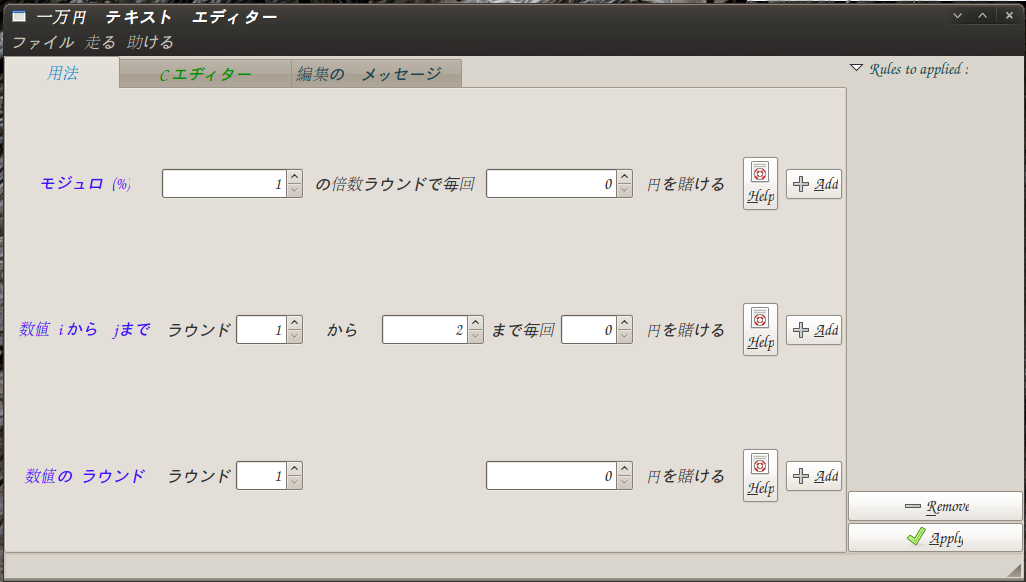
\includegraphics[height=25\baselineskip]{img/IDE.png}
\\\\\\
Execution Window:
\begin{center}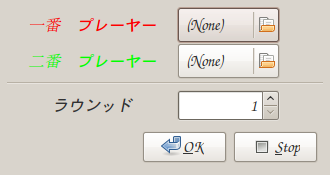
\includegraphics[height=10\baselineskip]{img/executing.png}\end{center}
\newpage
Execution Display Window:
\begin{center}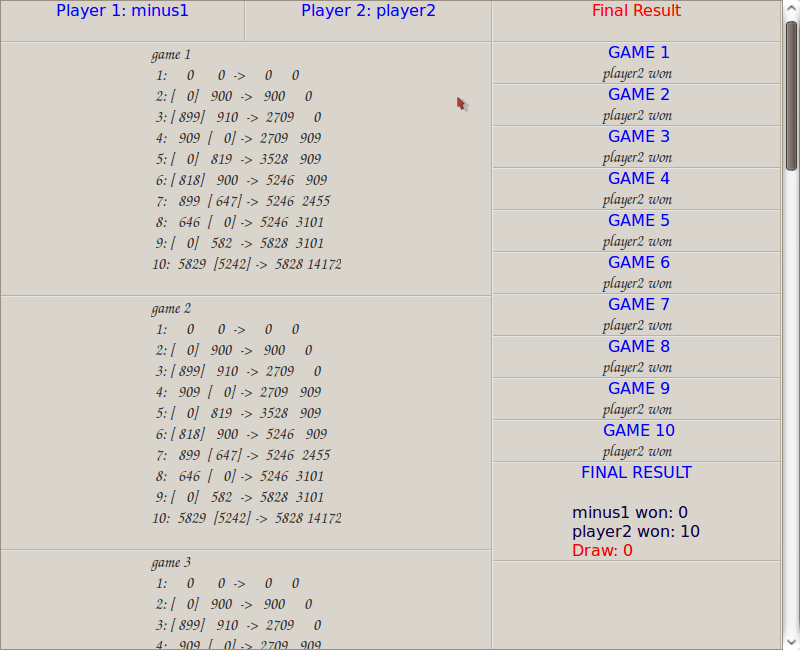
\includegraphics[height=28\baselineskip]{img/Display-program.png}\end{center}
\newpage
C Editor Notebook:
\begin{center}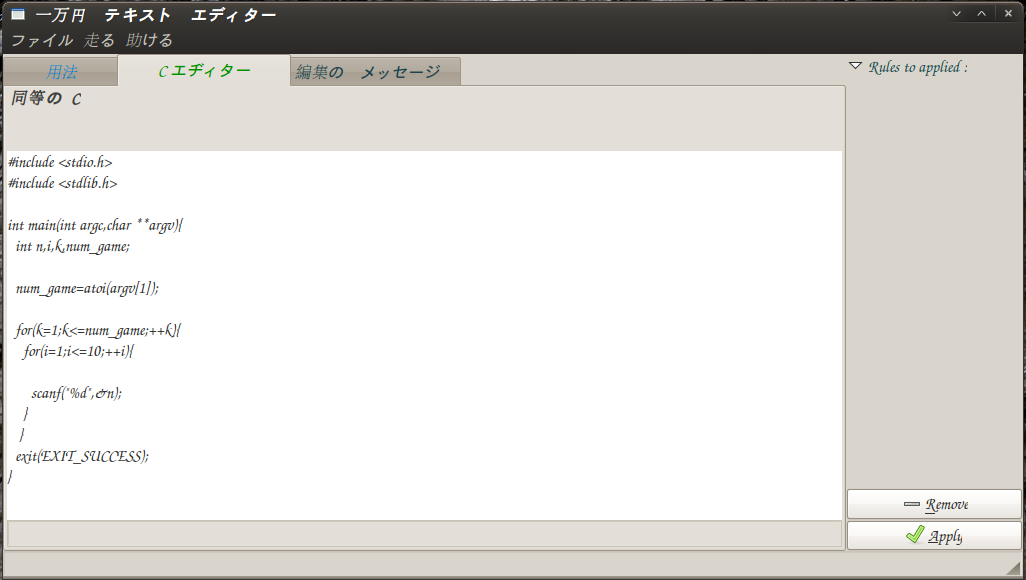
\includegraphics[height=20\baselineskip]{img/Editor.png}\end{center}
 Save a C file:
\begin{center}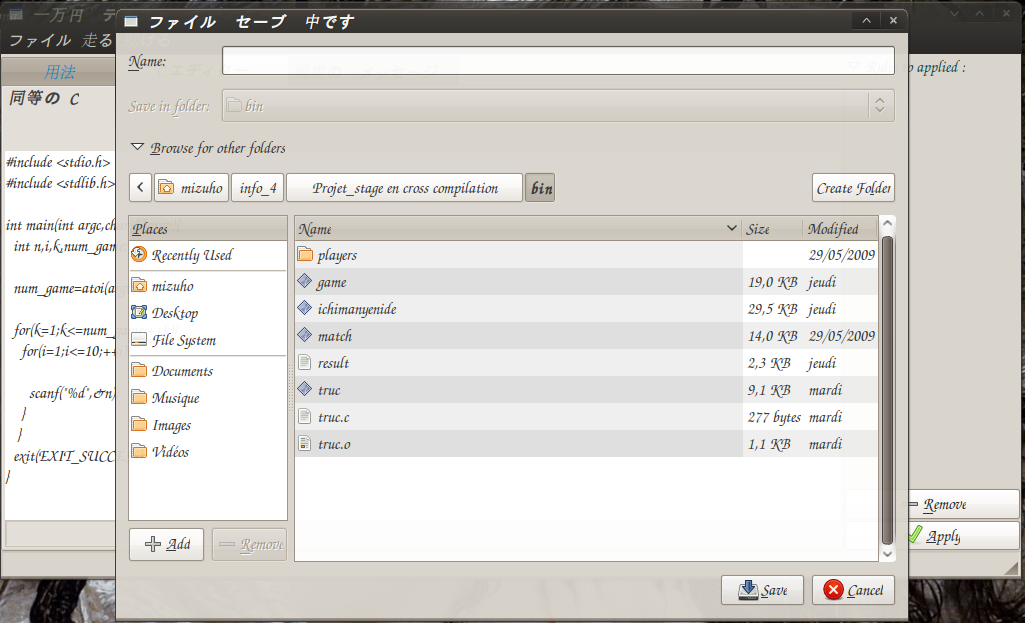
\includegraphics[height=20\baselineskip]{img/Saving-file.png}\end{center}\newpage
 Compile a C file:
\begin{center}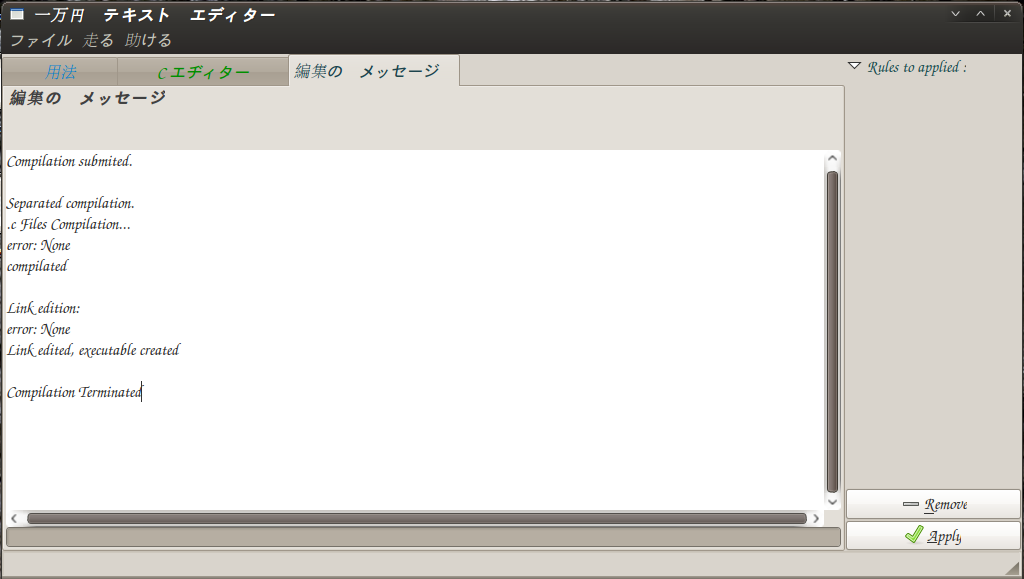
\includegraphics[height=20\baselineskip]{img/Compiler.png}\end{center}

\newpage
%################################################# Glossaire #############################################%


%\section*{Vocabulary \markboth{Vocabulary}{Vocabulary}}
%\addcontentsline{toc}{section}{\protect\numberline{}Vocabulary} \hspace{-7mm}
%\textcolor{Navy}{Pipe:} 





\newpage
%################################################ Extern sources Section #################################################%
\section*{Links / Documentation \markboth{Links / Documentation}{Links / Documentation}}
\addcontentsline{toc}{section}{\protect\numberline{}Links / Documentation}
\textcolor{Navy}{Japanese help links:}
\begin{verbatim}
   http://www.dictionnaire-japonais.com/
\end{verbatim}
\textcolor{Navy}{About Gtk Library}
\begin{verbatim}
   http://www.gtk-fr.org/
   http://www.gtk.org/
\end{verbatim}
\textcolor{Navy}{About CMake and cross-compilation}
\begin{verbatim}
   http://live.gnome.org/gtkmm/UsingCMake
   http://www.cmake.org/
\end{verbatim}
\textcolor{Navy}{Forums and community's programmers' website}
\begin{verbatim}
   http://www.siteduzero.com/
   http://www.developpez.com/
   http://www.codesources.com/
   http://www.commentcamarche.fr/
   http://www.ubuntu.com
\end{verbatim}
\textcolor{Navy}{About \LaTeX}
\begin{verbatim}
   http://www.latex-project.org/
\end{verbatim}
\textcolor{Navy}{And of course, the c "Man Pages" }
\begin{verbatim}
   http://www.linuxmanpages.com/
\end{verbatim}
\end{document}
